\section{Ranking}

Apparire nella prima pagina dei risultati di una ricerca è una cosa cruciale, il 95\% degli utenti non va oltre e in particolare il 51\% di ferma al primo risultato (al secondo classificato vanno il 16\% dei click, 5\% al terzo e ai restanti l'1\% tranne al 10 che si prende il 2\%).
Il punteggio di una pagina viene influenzato sia dal suo contenuto, sia da come è connessa con le altre pagine.

\subsection{TFIDF: Term Frequency - Inverse Document Frequency}

Viene calcolato per ogni keyword ed è basato sul contenuto della pagina, si calcola come il prodotto di due componenti:
\begin{itemize}
\item \textbf{TF} è la frequenza in percentuale con cui compare la keyword all'iterno della pagina
\item \textbf{IDF} è il logaritmo dell'inverso della frequenza della keyword (usato per non penalizzare eccessivamente le keyword complesse e poco frequenti)
\end{itemize}

\subsubsection{Aumentare il TFIDF}
Per aumentare il TFIDF basta inserire ripetutamente le keyword nella pagina.
Ci sono vari posti dove possono essere lette dai motori di ricerca:
\begin{itemize}
\item \textbf{Body Spam} le keyword vengono semplicemente inserite nel body della pagina HTML, sono visibili dall'utente quindi rovinano il conenuto
\item \textbf{Title Spam} le keyword vengono inserite nei titoli \texttt{<h1>, <h2>, ecc.}, è più vantaggioso dato che i motori di ricerca danno più importanza alle keyword nei titoli, inoltre il contenuto della pagina viene alterato marginalmente
\item \textbf{Meta Spam} le keyword vengono inserite nell'apposito meta tag, dato l'abuso di questa tecnica i motori di ricerca tendono a non considerarle.
\item \textbf{Anchor Spam} le keyword vengono inserite come testo di un link che punta alla pagina target, queste keyword vengono valutate di più dato che dovrebbero contenere un sommario della pagina che puntano. Es: \texttt{<a href=\"target.html\">free great deals, free, cheap</a>}
\item \textbf{URL Spam} le keyword vengono inserite nel URL della pagina. \\ Es: \texttt{http://buy-canon-rebel-t3.example.com} 
\end{itemize}
Generalmente queste tecniche di spamming vengono combinate.
In base a dove sono messe le keyword si hanno varie tecniche di spamming:
\begin{itemize}
\item \textbf{Repetition} determinate keyword vengono ripetute, è facilemente individuabile dai motori di ricerca
\item \textbf{Dumping} vengono inserite tante keyword in modo da rendere la pagina significativa per tante query, funziona bene con termini poco usati
\item \textbf{Weaving} vengono copiati articoli/news dal web nei quali si inseriscono delle keyword.
\item \textbf{Phrase Stitching} si attaccano frasi prese da siti diversi così facendo può essere che la pagina compaia nella SERP quando viene cercata una delle frasi
\item \textbf{Broadening} oltre alla keyword che si vuole spammare si usano anche i sinonimi. In questo modo oltre a coprire un range di keyword più vasto si guadagnano anche punti perchè keyword con lo stesso contesto sono ben viste dai motori di ricerca
\end{itemize}
Queste tecniche però rovinano l'aspetto della pagina, vengono quindi usati dei meccanismi di \textbf{Hiding} per preservare l'aspetto della pagina originale.
\begin{itemize}
\item \textbf{Content Hiding} la parte di testo riguardante le keyword viene resa invisibile usando come colore del testo lo stesso colore dello sfondo oppure usando la regola CSS \texttt{display:none;}.
Per nascondere i link si possono usare come ancora delle immagini trasparenti di 1x1 pixel.
\item \textbf{Redirection} una volta caricata la pagina con le keyword si reindirizza l'utente verso la pagina vera. Questo può essere fatto sia con del codice HTML sia con Javascript, conviene farlo con JS dato che i motori di ricerca fanno più fatica a comprenderlo
\item \textbf{Cloaking} simile al redirect, si basa sulla possibilità di distiunguere uno spider da un utente normale, quando la pagina viene richiesta da uno spider gli si fornisce quella contenete le keyword mentre quando viene richiesta da un utente gli si fornisce quella vera. L'identificazione può avvenire tramite indirizzo IP o con l'user-agent della richiesta HTTP.
\end{itemize}

\subsection{PageRank base}
Viene influenzato da come la pagina è connessa con il web e per questo influisce maggiormente nel calcolo complessivo.
La versione base del PageRank considera la rete come un grafo \textit{G(V,E)} dove i vertici sono le pagine web e gli spigoli sono i link tra le pagine.
Data quindi una pagina \textit{v} il suo PageRank è dato da:
$$ \pi_v = \sum_{(v,w) \in E} \frac{\pi_w}{d_w} $$
con
$$ \pi_v \geq 0 \ \forall v \in E $$ 
$$ \sum_v \pi_v = 1 $$
\begin{center}
$d_w$ numero di link uscenti dalla pagina $w$
\end{center}
Si possono però verificare delle situazioni in cui modificando i link uscenti di una pagina, il PageRank della pagina aumenti se le pagine erano collegate in modo circolare (A$\rightarrow$B, B$\rightarrow$C, C$\rightarrow$A se cambio A$\rightarrow$B in A$\rightarrow$C il PageRank di A aumenta).
Inoltre possono esserci gruppi di pagine isolate che rendono questa formulazione del PageRank non equa.

\subsubsection{PageRank} 
Per limitare il problemi del PageRank base si è presa in considerazione la possibilità di passare da una pagina all'altra anche senza passare per un link, con la formula:
$$ \pi_v = (1-\epsilon) ( \sum_{(v,w) \in E} \frac{\pi_w}{d_w} ) + \frac{\epsilon}{N} $$
dove $ \epsilon $ è la probabilità che si effettui un "teletrasporto" e N è il numero totale di pagine.
Anche questa versione soffre dei problemi del PageRank base però ne è meno vulnerabile dato che il PageRank di una pagina non può mai essere 0.
Da notare che se $\epsilon=0$ si torna al PageRank base e se $\epsilon=1$ ogni pagina ha lo stesso PageRank.

\subsubsection{Aumentare il PageRank}

Aggiungere link in ingresso ad una pagina aumenta sempre il PageRank.
Ci sono varie tecniche:
\begin{itemize}
\item \textbf{Infiltration} ci si infiltra in altri siti per aggiungere InLink verso la propria pagina, per esempio sfruttando delle Wiki o i commenti di un blog
\item \textbf{Honey Pot} si inserisce del contenuto interessante (anche copia-incollato) nella pagina, sperando che altri siti si riferiscano a noi
\item \textbf{Link Exchange} ci si accorda con altri siti per linkarsi reciprocamente
\item \textbf{Ressurrection} si compra un dominio scaduto recentemente e si crea una pagina con un link al nostro sito, in questo modo se il dominio aveva dei link entrati questi aumenteranno il PageRank del nostro sito
\end{itemize}

\subsubsection{Spam Farm}
Una spam farm è una struttura di pagine creata con lo scopo di aumentare il PageRank di una pagina target.
Si è dimostrato che, perché una spam farm sia ottima devono valere le seguenti condizioni:
\begin{itemize}
\item Tutte le \textit{boosting pages} abbiamo link uscenti solamente verso la pagina target
\item Non ci siano link tra le \textit{boosting pages}
\item La pagina target abbia link almeno verso una \textit{boosting page}
\item Tutti i link \textit{hijacked} siano verso la pagina Target
\end{itemize}
Il terzo punto è particolarmente importante perché se le \textit{boosting pages} non vengono raggiunte dallo spider dei motori di ricerca non contribuiscono ad aumentare il PageRank della pagina target (\textbf{Reachability}).

\begin{figure}
\centering
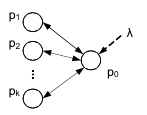
\includegraphics{images/spamfarm_ottima.png}
\caption{Spam Farm Ottima}\label{fig:1}
\end{figure}
Più spam farm possono anche avere link tra loro creano delle \textbf{Spam Farm Alliance}, queste alleanze possono essere di due tipi:
\begin{itemize}
\item \textbf{Alleanze Profonde} le boosting pages di tutte le spam farm dell'alleanza puntano a tutte le pagine target presenti nell'alleanza, se l'alleanza è composta da due spam farm il PageRank delle pagine target diventa la media del PageRank che avevano in precedenza
\item \textbf{Alleanze Superiori} le pagine target dell'alleanza sono tra loro linkate, se l'alleanza è composta solamente da due spam farm il PageRank di entrambe le pagine diventa uguale al massimo dei PageRank precedenti. Le alleanze superiori tra più spam farm possono essere a \textbf{Ring} o \textbf{Complete Core}.
\end{itemize}

\begin{figure}
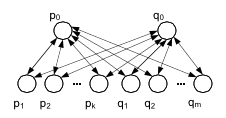
\includegraphics{images/alleanza_profonda.png}
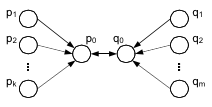
\includegraphics{images/alleanza_sup.png}
\caption{A sinistra: Alleanza Profonda, A destra: Alleanza Superiore}\label{fig:2}
\end{figure}
I motori di ricerca nel tempo hanno adottato delle contro misure, per esempio, per ogni pagina possono calcolare sia il PageRank Base sia quello con "teletrasporto" e calcolarne la differenza (\textbf{Massa di Spam}), se la differenza è notevole analizzano la struttura per vedere se rispecchia la struttura media del web, se trovano una struttura diversa penalizzano il sito (il 95\% dei siti con un'elevata massa di spam sono effettivamente delle spam farm).

\subsubsection{\#Janus Graph}
Il web viene visto come un grafo bipesato, ogni nodo ha un ranking positivo $W+$ e uno negativo $W-$.
La parte positiva viene calcolata con un sistema di ranking qualsiasi, per esempio il PageRank mentre per quella negativa si usa un PageRank basato sull'idea che la parte negativa è duale e opposta: i link vengono "girati" in modo da penalizzare le pagine web che linkano pagine "negative".
$$ R^J = R(G^+) - R((G^R)^-) $$
Per valutare la parte negativa possono anche basarmi su strutture informative già esistenti quali le email.

